\documentclass[c,unicode,russian]{beamer}
\usepackage{hyperref}
\usepackage{alltt}
\usepackage{verbatim}
\usepackage{fancyvrb}

\usepackage{fontspec}
\setsansfont{Ubuntu}
\setmonofont{Ubuntu Mono}
\usepackage{polyglossia}
\setdefaultlanguage{russian}

\useinnertheme{metropolis}
\useoutertheme{metropolis}
\usecolortheme{metropolis}

\usepackage{listings}   % C++ code
\usepackage{xcolor}     % C++ code
\lstset{%
    keywordstyle=\color{blue},
    commentstyle=\color[rgb]{0.13,0.54,0.13},
    backgroundcolor=\color{yellow!10},
    basicstyle=\small\tt,
    stringstyle=\color{red}\ttfamily,
    belowcaptionskip=-1pt,
    xleftmargin=-15pt,
    framexleftmargin=-15pt,
    framexrightmargin=5pt,
    framextopmargin=5pt,
    framexbottommargin=5pt,
    framesep=0pt,
    rulesep=0pt
}
\lstdefinestyle{cpp}{%
    language=C++,
    morecomment=[l][\color{magenta}]{\#}
}
\lstdefinestyle{python}{%
    language=Python
}

\usepackage{caption}
\renewcommand{\lstlistingname}{Код} % Listing -> Algorithm
\DeclareCaptionFont{white}{\color{white}}
\DeclareCaptionFormat{listing}{\colorbox{gray}{\parbox{\textwidth}{#1#2#3}}}
\captionsetup[lstlisting]{format=listing,labelfont=white,textfont=white}

% logo of my university
\titlegraphic{\hspace{-1cm}
\includegraphics[width=2.5in]{../../_static/logo.jpg}}

\date{}
\author{Основы Веб-программирования}
\institute{Кафедра Интеллектуальных Информационных Технологий, ИнФО, УрФУ}

\usepackage{array}      % Table
\usepackage{dirtytalk}  % say
\usepackage{tabularx}

\title{Веб без фреймворков}

\begin{document}

% Slide #1
\frame{\titlepage}

% Slide #2
\begin{frame}{Ресурсы}
  \url{http://lectures.uralbash.ru/6.www.sync/2.codding/index.html}
\end{frame}

% Slide #3
\begin{frame}{WSGI - это\ldots?}

    Для разработки сайтов или Web-приложений на языке Python был утверждён
    стандарт взаимодействия между Python-приложениями и сервером (например
    Apache), названный WSGI (“Web Server Gateway Interface”).

    \textbf{Python}\newline
    \textbf{pep-333}\newline
    \textbf{pep-3333}\newline

\end{frame}

% Slide #4
\begin{frame}{Общие принципы}

  \begin{itemize}
    \item Веб-сервер
    \item Разделение кода: \textbf{MVC}, \textbf{MTV}, \textbf{RV}
    \item Маршрутизация URL
    \item Шаблоны
    \item Пагинация
    \item Request/Response
    \item Статика
    \item Формы
  \end{itemize}

\end{frame}


% Slide #7
\begin{frame}{Веб-сервер}

  \textbf{Веб сервер}

\end{frame}


% Slide #5
\begin{frame}{Веб-сервер}

  Задача Веб сервера - запускать Веб приложения.\newline\newline
    Популярные WSGI Веб сервера:\newline

  \begin{itemize}
    \item wsgiref
    \item Paste
    \item Waitress
    \item Gunicorn
  \end{itemize}


\end{frame}

% Slide #6
\begin{frame}[fragile]{wsgiref}

    \begin{lstlisting}[style=python]
    from wsgiref.simple_server import make_server

    def hello_world_app(environ, start_response):
        status = '200 OK'  # HTTP Status
        headers = [
          ('Content-type', 'text/plain; charset=utf-8')
        ]  # HTTP Headers
        start_response(status, headers)

        # The returned object is going to be printed
        return [b"Hello World"]

    with make_server('', 8000, hello_world_app) as httpd:
        print("Serving on port 8000...")

        # Serve until process is killed
        httpd.serve_forever()
    \end{lstlisting}

\end{frame}


% Slide #7
\begin{frame}{Разделение кода: \textbf{MVC}, \textbf{MTV}, \textbf{RV}}

  \textbf{Разделение кода на части}

\end{frame}


% Slide #7
\begin{frame}{Разделение кода: \textbf{MVC}}

  \textbf{MVC} (Model-View-Controller: модель-вид-контроллер) —

  шаблон архитектуры ПО, который подразумевает разделение программы на 3
  слабосвязанных компонента, каждый из которых отвечает за свою сферу
  деятельности.

\end{frame}


% Slide #8
\begin{frame}{Разделение кода: \textbf{MVC}}

  \begin{center}
    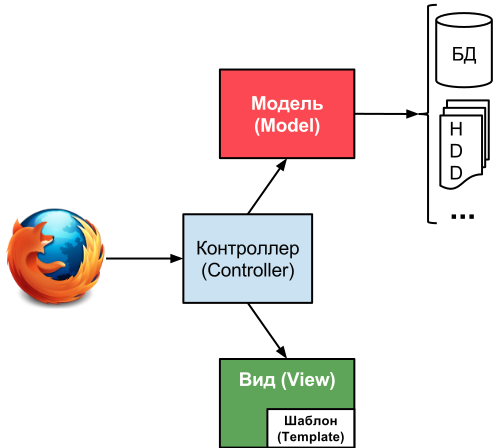
\includegraphics[width=3.2in]{media/mvc.png}
  \end{center}

\end{frame}


% Slide #9
\begin{frame}{Разделение кода: \textbf{MVC}}

  Классические \textbf{MVC} фреймворки:

  \begin{itemize}
    \item Ruby on Rails
    \item Pylons
  \end{itemize}

\end{frame}


% Slide #8
\begin{frame}{Разделение кода: \textbf{MTV}}

  Фреймворк \textbf{Django} ввел новую терминологию \textbf{MTV}

  \begin{itemize}
    \item \textbf{M -> M} Модели остались неизменными
    \item \textbf{V -> T} Представление назвали Templates
    \item \textbf{C -> V} Контроллеры назвали Views
  \end{itemize}

\end{frame}


% Slide #8
\begin{frame}{Разделение кода: \textbf{MTV}}

  Tada! Django MTV

  \begin{center}
    
\includegraphics[width=2.2in]{media/mtv_logo.jpg}
  \end{center}

\end{frame}

% Slide #8
\begin{frame}{Разделение кода: \textbf{MTV}}

  \begin{center}
    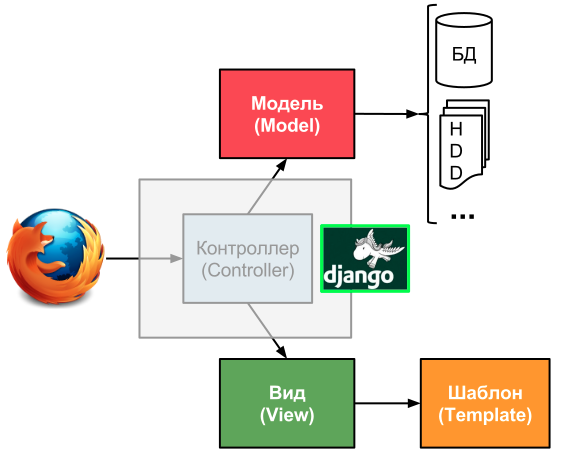
\includegraphics[width=3.2in]{media/mtv.png}
  \end{center}

\end{frame}

% Slide #11
\begin{frame}{Разделение кода: \textbf{MVC}, \textbf{MTV}, \textbf{RV}}

  Разработка без фреймворков дает вам возможность придерживаться любой
  архитектуры приложения и паттерна проектирования.

\end{frame}

% Slide #12
\begin{frame}{Разделение кода: \textbf{MVC}, \textbf{MTV}, \textbf{RV}}

  Это дает неоспоримую гибкость таким приложениям, оставляя ответственность по
  структуре ПО за разработчиком.

\end{frame}


% Slide #10
\begin{frame}{Разделение кода: \textbf{RV}}

  \textbf{RV} (Resources-View) --

  дает ту же гибкость, накладывая минимальную архитектуру идеально
  вписывающуюся в ограничения Веб приложений.

\end{frame}


% Slide #8
\begin{frame}{Разделение кода: \textbf{RV}}

  \begin{center}
    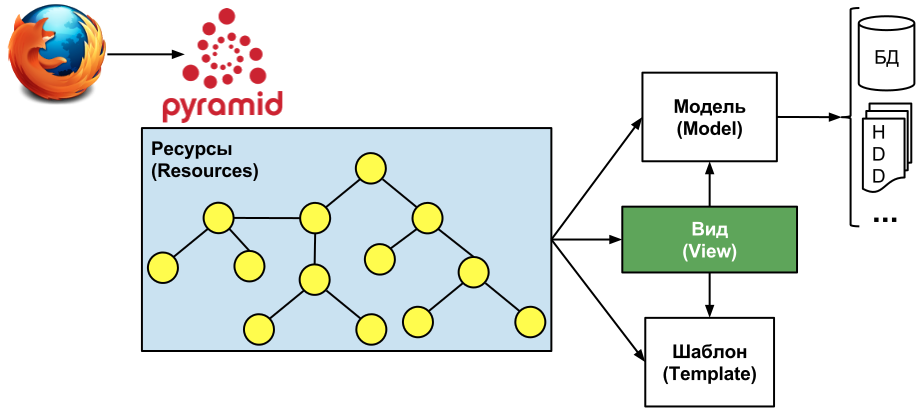
\includegraphics[width=4.0in]{media/rv.png}
  \end{center}

\end{frame}


% Slide #10
\begin{frame}{Разделение кода: \textbf{RV}}

  \say{Мы считаем, что есть только две вещи: ресурсы (\textbf{Resource}) и
    виды (\textbf{View}). Дерево ресурсов представляет структуру сайта, а вид
    представляет ресурс.
  }

\end{frame}

% Slide #10
\begin{frame}{Разделение кода: \textbf{RV}}

  \say{«\textbf{Шаблоны}» (\textbf{Template}) в реальности лишь
    деталь реализации некоторого вида: строго говоря, они не обязательны, и вид
    может вернуть ответ (Response) и без них.
  }

\end{frame}

% Slide #10
\begin{frame}{Разделение кода: \textbf{RV}}

  \say{Нет никакого «\textbf{Контроллера}» (\textbf{controller}): его просто не
    существует. «\textbf{Модель}» (\textbf{Model}) же либо представлена деревом
    ресурсов, либо «доменной моделью» (domain model) (например, моделью
    \textbf{SQLAlchemy}), которая вообще не является частью каркаса. Нам
    кажется, что наша терминология более разумна при существующих ограничениях
    веб-технологий.
  }

\end{frame}


% Slide #10
\begin{frame}{Разделение кода: \textbf{RV}}

  \textbf{Pyramid} only

    
\includegraphics[width=0.5in]{media/pyramid.png}

\end{frame}

% Slide #7
\begin{frame}{Маршруты}

  \textbf{Маршруты}

  или

  \textbf{Диспетчеризация URL}

\end{frame}

% Slide #8
\begin{frame}{Маршруты: Сортировочная Ж/Д станция}

  \begin{center}
    \vspace{-20pt}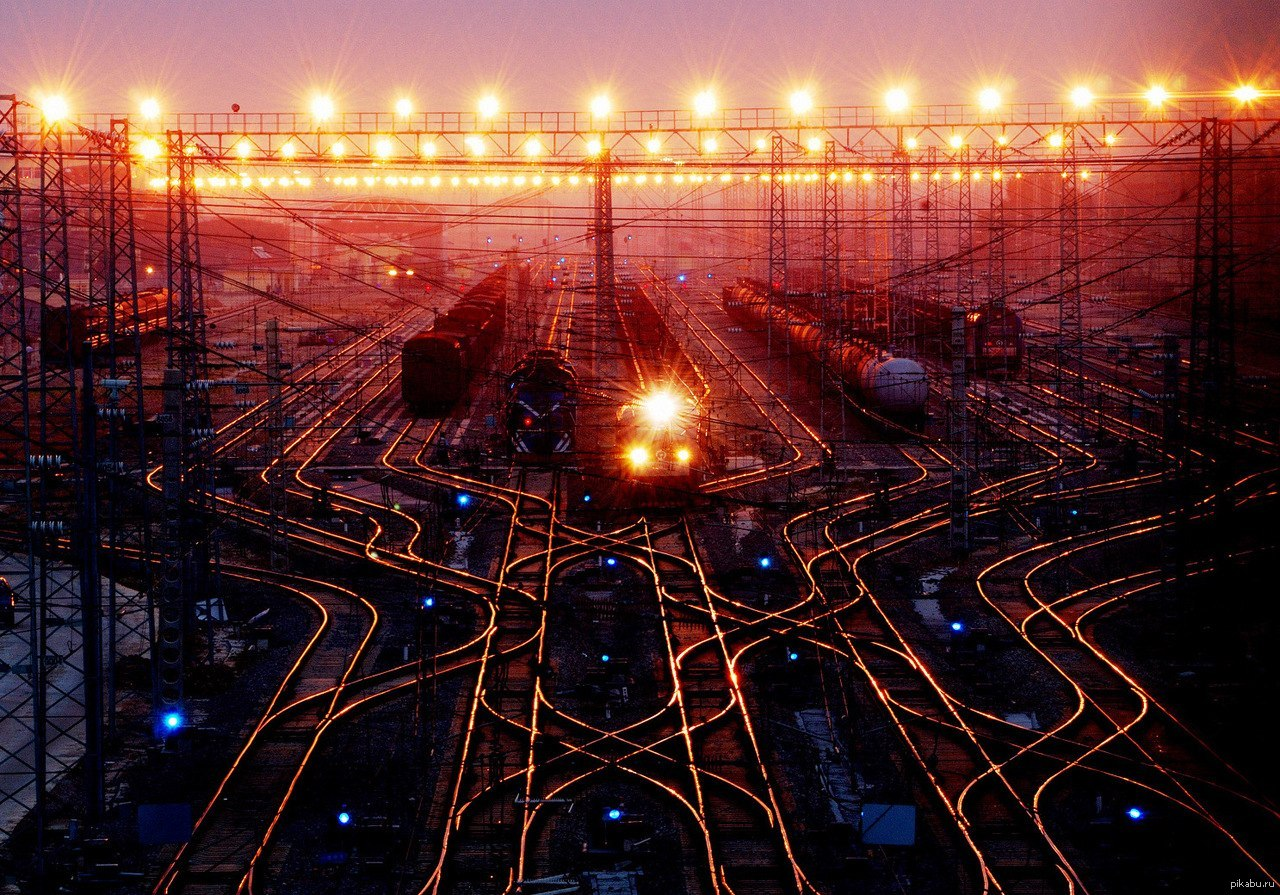
\includegraphics[width=\textwidth,height=\textheight,keepaspectratio]{media/routes.jpg}
  \end{center}

\end{frame}


% Slide #8
\begin{frame}{Маршруты: Сортировочная Ж/Д станция}

  \begin{itemize}
    \item \textbf{Поезда} похожи на HTTP запросы клиентов
    \item \textbf{Сортировочная станция} представляет из себя
      \textbf{маршруты}, только вместо поездов занимается диспетчеризацией HTTP
      запросов от клиентов
    \item \textbf{Пункт назначения} (завод или вокзал) можно сравнить с
      функцией (кодом), которая обрабатывает запрос
  \end{itemize}

\end{frame}


% Slide #8
\begin{frame}{Маршруты: Определение}

  \textbf{Маршруты} определяют шаблоны URL и связывают их со своим кодом

\end{frame}


% Slide #8
\begin{frame}{Маршруты: Преимущества}

  В отличии от CGI, где все привязано к файловой системе,
  если вы измените свое решение по поводу конкретного URL, то просто поменяйте
  шаблон URL - код по-прежнему будет работать отлично и не понадобится менять
  какую-либо логику.

\end{frame}

% Slide #8
\begin{frame}[fragile]{Маршруты: Регулярные выражения}

  \begin{lstlisting}[style=python]
    from django.conf.urls import url

    from . import views

    urlpatterns = [
     url(r'^articles/2003/$', views.special_case_2003),
     url(r'^articles/([0-9]{4})/$', views.year_archive),
     url(r'^articles/([0-9]{4})/([0-9]{2})/$', views.month_archive),
     url(r'^articles/([0-9]{4})/([0-9]{2})/([0-9]+)/$', views.article_detail),
    ]
    \end{lstlisting}

\end{frame}

% Slide #8
\begin{frame}[fragile]{Маршруты: Django 2.0 - Сопоставление с образом}

  \begin{lstlisting}[style=python]
    from django.urls import path

    from . import views

    urlpatterns = [
      path('articles/2003/', views.special_case_2003),
      path('articles/<int:year>/', views.year_archive),
      path('articles/<int:year>/<int:month>/', views.month_archive),
      path('articles/<int:year>/<int:month>/<slug:slug>/', views.article_detail),
    ]
    \end{lstlisting}

\end{frame}

% Slide #8
\begin{frame}[fragile]{Маршруты: Сопоставление с образом}

  \begin{lstlisting}[style=python]
    import selector

    dispatch = selector.Selector()
    dispatch.add('/', GET=BlogIndex)
    dispatch.add('/add', GET=create, POST=create)
    dispatch.add('/{id:digits}', GET=BlogRead)
    dispatch.add('/{id:digits}/edit', GET=update, POST=update)
    dispatch.add('/{id:digits}/delete', GET=delete)
  \end{lstlisting}

\end{frame}





\begin{frame}[fragile]{Маршруты: Сравнение}

  \begin{table}[]
  \centering
  \label{my-label}
  \begin{tabular}{ll}
    Регулярные выражения & Сопоставление с образом \\
    / & / \\
    /article/add & /article/add \\
    \verb|^/article/(?P<id>d+)/$|       & \verb|/article/{id:digits}|      \\
    \verb|^/article/(?P<id>d+)/edit$|   & \verb|/article/{id:digits}/edit| \\
    \verb|^/article/(?P<id>d+)/delete$| & \verb|/article/{id:digits}/delete|

  \end{tabular}
  \end{table}

\end{frame}

% Slide #8
\begin{frame}{Маршруты: Преимущества}

  \begin{itemize}
    \item
      Регулярные выражения дают огромные возможности.
    \item
      Но из-за ограничений \newline
      описанных в стандарте RFC 1738,
      большинство из них не нужны.
    \item
      Использование регулярных выражений затрудняет читабельность кода.
  \end{itemize}

\end{frame}


% Slide #8
\begin{frame}{Шаблоны}

  \textbf{Шаблоны}

\end{frame}


% Slide #8
\begin{frame}{Шаблоны: Определение}

  \textbf{Шаблоны} имеют очень простое определение - в статические файлы вставляются
  куски кода, при прогоне таких файлов через специальный транслятор
  (препроцессор), код заменяется результатом его выполнения.

\end{frame}


% Slide #8
\begin{frame}[fragile]{Шаблоны: C++}

  \begin{lstlisting}[style=cpp]
    template< typename T >
    T min( T a, T b )
    {
      return a < b ? a : b;
    }
  \end{lstlisting}

  \begin{lstlisting}[style=cpp]
    int min( int a, int b )
    {
      return a < b ? a : b;
    }

    long min( long a, long b )
    {
      return a < b ? a : b;
    }
  \end{lstlisting}

\end{frame}

% Slide #8
\begin{frame}[fragile]{Шаблоны: PHP}

  \begin{lstlisting}[style=php]
  <html>
    <head> <title> Тестируем PHP </title> </head>
    <body>
    <?php
      echo '<h1>Hello, world!</h1>';
    ?>
    <br />
    <?php
      $colors = array("red", "green", "blue", "yellow");

      foreach ($colors as $value) {
          echo "* $value <br />\n";
      }
    ?>
    </body>
  </html>
  \end{lstlisting}

\end{frame}

% Slide #8
\begin{frame}[fragile]{Шаблоны: PHP}

  \begin{lstlisting}[style=html]
    <body>

    <h1>Hello, world!</h1>
    <br />

    * red <br />
    * green <br />
    * blue <br />
    * yellow <br />

    </body>
  \end{lstlisting}

\end{frame}

% Slide #8
\begin{frame}{Шаблоны: Jinja2}

  \textbf{Jinja2} — самый популярный шаблонизатор в языке программирования
  Python. Автор Armin Ronacher из команды http://www.pocoo.org/, не раз
  приезжал на конференции в Екатеринбург с докладами о своих продуктах.

\end{frame}


% Slide #8
\begin{frame}{Шаблоны: Jinja2}

  \begin{center}
    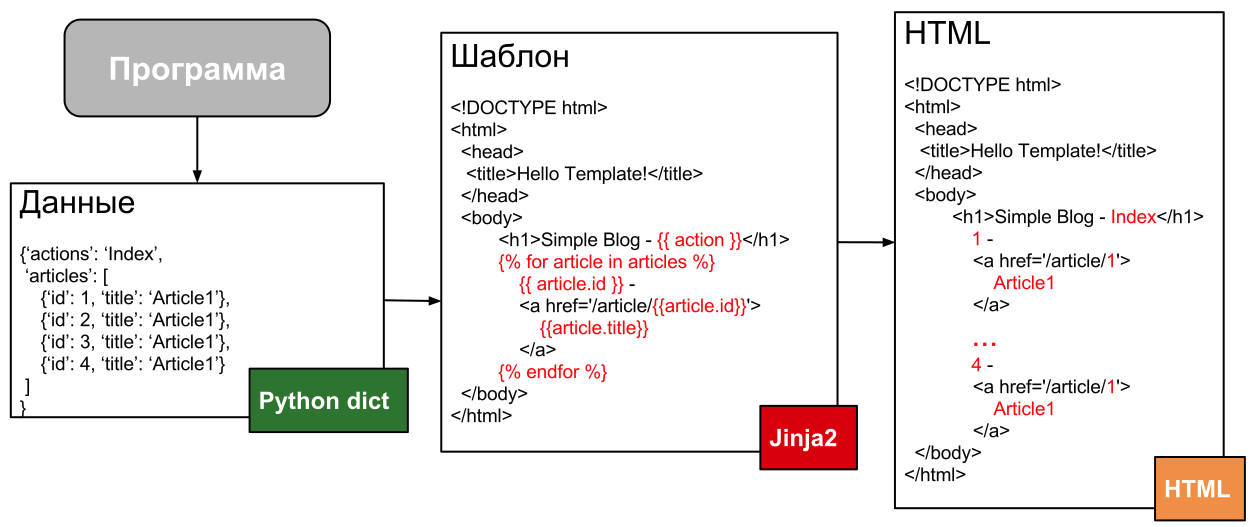
\includegraphics[width=\textwidth,height=\textheight,keepaspectratio]{media/template.png}
  \end{center}

\end{frame}

% Slide #8
\begin{frame}[fragile]{Шаблоны: Jinja2 - \{\{ выражения \}\}}

  \begin{lstlisting}[style=Python]
    from jinja2 import Template

    template = Template('Hello {{ name }}!')
    print(template.render(name='Вася'))
  \end{lstlisting}

  Hello Вася!

\end{frame}

% Slide #8
\begin{frame}[fragile]{Шаблоны: Jinja2 - \{\# комментарии \#\}}

  \begin{lstlisting}
    {# Это кусок кода
       который стал временно не ненужен,
       но удалять жалко
        
            ...
        
    #}
  \end{lstlisting}

\end{frame}

% Slide #8
\begin{frame}[fragile]{Шаблоны: Jinja2 - \{\% операторы \%\}}

  \begin{lstlisting}[style=Python]
    from jinja2 import Template
    text = ''
      'Hello {{ name }}! '
    template = Template(text)
    print(template.render(name='Вася'))
  \end{lstlisting}

  Hello Вася! Hello Вася! Hello Вася! Hello Вася! Hello Вася!

\end{frame}

% Slide #8
\begin{frame}[fragile]{Шаблоны: Jinja2 - модули}

  \begin{lstlisting}[style=Python]
    from jinja2 import Template
    template = Template(
      ""
    )
    m = template.module
    print(m.a)
    print(m.b)
    print(m.c)
  \end{lstlisting}

  foo\newline
  фуу\newline
  föö

\end{frame}

% Slide #8
\begin{frame}[fragile]{Шаблоны: Jinja2 - чтение из файла}

  \begin{lstlisting}[style=html]
    <!DOCTYPE html>
    <html>
      <head>
        <meta http-equiv="Content-Type" content="text/html; charset=utf-8" />
      </head>
      <body>
        
          Hello {{ name }}!
        
      </body>
    </html>
  \end{lstlisting}

\end{frame}

% Slide #8
\begin{frame}[fragile]{Шаблоны: Jinja2 - чтение из файла}

  \begin{lstlisting}[style=python]
    from jinja2 import Template

    html = open('foopkg/templates/0.hello.html').read()
    template = Template(html)
    print(template.render(name='Петя'))
  \end{lstlisting}

\end{frame}

% Slide #8
\begin{frame}[fragile]{Шаблоны: Jinja2 - чтение из файла}

  \begin{lstlisting}[style=html]
    <!DOCTYPE html>
    <html>
      <head>
        <meta http-equiv="Content-Type" content="text/html; charset=utf-8" />
      </head>
      <body>

          Hello Петя!

          Hello Петя!

          Hello Петя!

          Hello Петя!

          Hello Петя!

      </body>
    </html>
  \end{lstlisting}

\end{frame}

% Slide #8
\begin{frame}[fragile]{Шаблоны: Jinja2 - \{\% extends "наследование" \%\}}

  \begin{lstlisting}[style=html]
    <head>
        
          <link rel="stylesheet" href="style.css" />
          <title>
             - My Webpage</title>
          <meta charset='utf-8'>
        
    </head>
    <body>
        <div id="content">
          </div>
        <div id="footer">
            
              &copy; Copyright 2008 by
              <a href="http://domain.invalid/">you</a>.
            
        </div>
    </body>
  \end{lstlisting}

\end{frame}

% Slide #8
\begin{frame}[fragile]{Шаблоны: Jinja2 - \{\% extends "наследование" \%\}}

  \begin{lstlisting}[style=html]
    
    Index
    
        {{ super() }}
        <style type="text/css">
            .important { color: #336699; }
        </style>
    
    
        <h1>Index</h1>
        <p class="important">
          Welcome {{ name }} to my awesome homepage.
        </p>
    
  \end{lstlisting}

\end{frame}


% Slide #8
\begin{frame}[fragile]{Шаблоны: Jinja2 - \{\% extends "наследование" \%\}}

  \begin{lstlisting}[style=python]
    from jinja2 import Environment, FileSystemLoader

    env = Environment(loader=FileSystemLoader('.'))
    template = env.get_template('index.html')
    print(template.render(name='Петя'))
  \end{lstlisting}

\end{frame}

% Slide #8
\begin{frame}[fragile]{Шаблоны: Jinja2 - \{\% extends "наследование" \%\}}

  \begin{lstlisting}[style=python]
    <!DOCTYPE html>
    <html lang="en">
    <head>


        <link rel="stylesheet" href="style.css" />
        <title>Index - My Webpage</title>
        <meta charset='utf-8'>

        <style type="text/css">
            .important { color: #336699; }
        </style>

    </head>
  \end{lstlisting}

\end{frame}

% Slide #8
\begin{frame}[fragile]{Шаблоны: Jinja2 - \{\% extends "наследование" \%\}}

  \begin{lstlisting}[style=python]
    <body>
        <div id="content">
        <h1>Index</h1>
        <p class="important">
          Welcome Петя to my awesome homepage.
        </p>
    </div>
        <div id="footer">

            &copy; Copyright 2008 by <a href="http://domain.invalid/">you</a>.

        </div>
    </body>
    </html>
  \end{lstlisting}

\end{frame}

% Slide #8
\begin{frame}{Пагинация}

  \textbf{Пагинация}

\end{frame}


% Slide #8
\begin{frame}{Пагинация: Определение}

  \textbf{Пагинация} --- разделение контента на страницы.

\end{frame}

% Slide #8
\begin{frame}{Пагинация: www.opennet.ru}

  \begin{center}
    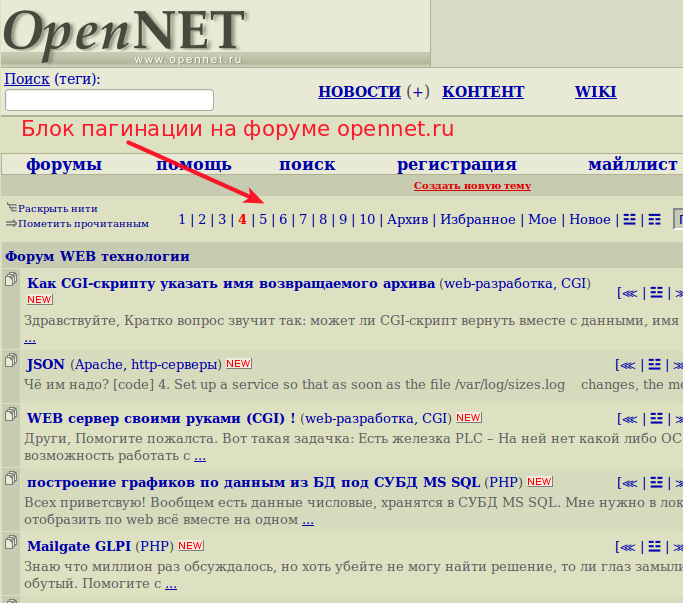
\includegraphics[width=\textwidth]{media/opennet.png}
  \end{center}

\end{frame}

\begin{frame}{Пагинация: market.yandex.ru}

  \begin{center}
    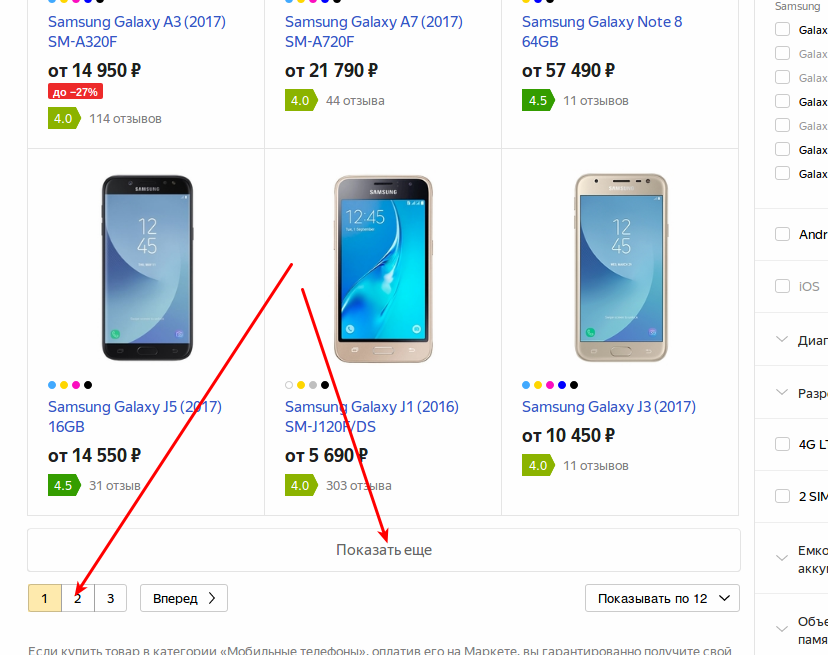
\includegraphics[width=\textwidth]{media/yandex-market-pagination.png}
  \end{center}

\end{frame}

% Slide #8
\begin{frame}{Пагинация: Python}

  pip install \textbf{paginate}

  https://github.com/Pylons/paginate

\end{frame}

% Slide #8
\begin{frame}[fragile]{Пагинация: Python}

  \begin{lstlisting}[style=python]
      from paginate import Page
      page = values.get('page', 1)
      paged_articles = Page(
          ARTICLES,
          page=page,
          items_per_page=8,
      )
  \end{lstlisting}

\end{frame}

% Slide #8
\begin{frame}[fragile]{Пагинация: Python}

  \begin{lstlisting}[style=python]
    
      <div class="blog-list__item">
        <div class="blog-list__item-id">
        {{ article.id }}</div>
        <a href="/article/{{ article.id }}"
          class="blog-list__item-link">{{ article.title }}</a>
        <div class="blog-list__item-action">
          <a href="/article/{{ article.id }}/edit"
            class="blog-list__item-edit">edit</a>
          <a href="/article/{{ article.id }}/delete"
            onclick="return confirm_delete();"
            class="blog-list__item-delete">delete</a>
        </div>
      </div>
    
  \end{lstlisting}

\end{frame}

% Slide #8
\begin{frame}[fragile]{Пагинация: Python}

  \begin{lstlisting}[style=python]
    <div class="paginator">
        {{ articles.pager(url="?page=$page") }}
    </div>
  \end{lstlisting}

\end{frame}


\begin{frame}{Пагинация: Python}

  \begin{center}
    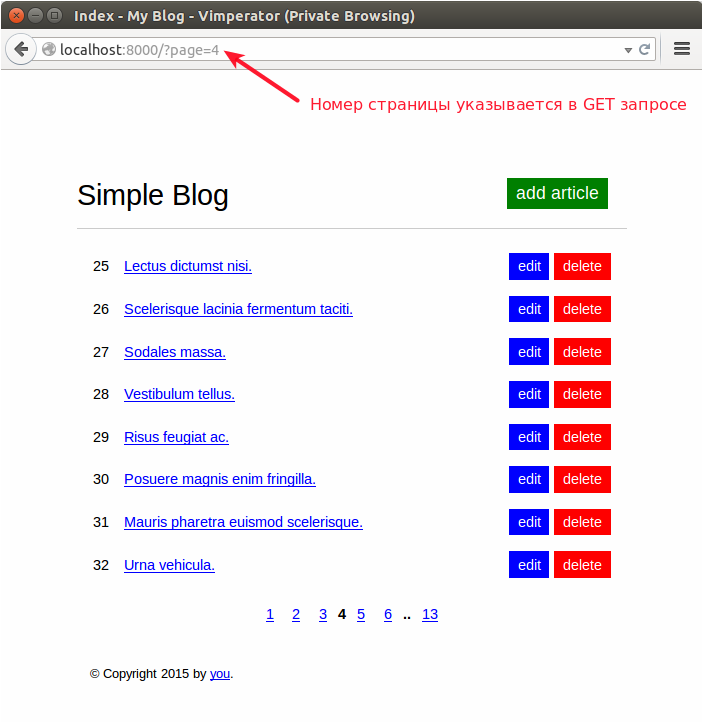
\includegraphics[height=\textheight]{media/blog_with_page.png}
  \end{center}

\end{frame}

% Slide #8
\begin{frame}{Request/Response. WebOb}

  \textbf{WebOb} --- библиотека сериализующая HTTP запрос (текст) в объект и
  наоборот объект в HTTP ответ (текст).

\end{frame}

% Slide #8
\begin{frame}[fragile]{WebOb. Сравнение}

  http://localhost:80/blog?page=42

  \begin{lstlisting}[style=python]
    from urlparse import parse_qs

    values = parse_qs(environ['QUERY_STRING'])
    page = values.get('page', ['1', ]).pop()
  \end{lstlisting}

  \begin{lstlisting}[style=python]
    from webob import Request

    req = Request(environ)
    page = req.params.get('page', '1')
  \end{lstlisting}

\end{frame}


% Slide #8
\begin{frame}[fragile]{WebOb. Request из окружения}

  \begin{lstlisting}[style=python]
    environ = {
        'HTTP_HOST': 'localhost:80',
        'PATH_INFO': '/article',
        'QUERY_STRING': 'id=1',
        'REQUEST_METHOD': 'GET',
        'SCRIPT_NAME': ''
    }

    from webob import Request
    req = Request(environ)
  \end{lstlisting}

\end{frame}

% Slide #8
\begin{frame}[fragile]{WebOb. Request Mock}

  \begin{lstlisting}[style=python]
    from webob import Request
    req = Request.blank('/blog?page=4')

    from pprint import pprint
    pprint(req.environ)
  \end{lstlisting}

\end{frame}


% Slide #8
\begin{frame}[fragile]{WebOb. Request Mock}

  \begin{lstlisting}[style=python]
    {'HTTP_HOST': 'localhost:80',
     'PATH_INFO': '/blog',
     'QUERY_STRING': 'page=4',
     'REQUEST_METHOD': 'GET',
     'SCRIPT_NAME': '',
     'SERVER_NAME': 'localhost',
     'SERVER_PORT': '80',
     'SERVER_PROTOCOL': 'HTTP/1.0',
     'wsgi.errors': <open file '<stderr>', mode 'w' at 0x7f4ff5d111e0>,
     'wsgi.input': <_io.BytesIO object at 0x7f4ff3b622f0>,
     'wsgi.multiprocess': False,
     'wsgi.multithread': False,
     'wsgi.run_once': False,
     'wsgi.url_scheme': 'http',
     'wsgi.version': (1, 0)}
  \end{lstlisting}

\end{frame}

% Slide #8
\begin{frame}[fragile]{WebOb. Request методы}

  \begin{lstlisting}[style=python]
    from webob import Request
    req = Request.blank('/blog?page=4')

    print(req.method)
    print(req.scheme)
    print(req.path_info)
    print(req.host)
    print(req.host_url)
    print(req.application_url)
    print(req.path_url)
    print(req.url)
    print(req.path)
    print(req.path_qs)
    print(req.query_string)
  \end{lstlisting}

\end{frame}


% Slide #8
\begin{frame}[fragile]{WebOb. Request методы}

  \begin{lstlisting}[style=python]
    GET
    http
    /blog
    localhost:80
    http://localhost
    http://localhost
    http://localhost/blog
    http://localhost/blog?page=4
    /blog
    /blog?page=4
    page=4
  \end{lstlisting}

\end{frame}

% Slide #8
\begin{frame}[fragile]{WebOb. Request GET}

  \begin{lstlisting}[style=python]
    from webob import Request
    req = Request.blank('/test?check=a&check=b&name=Bob')

    print(req.GET)
    print(req.GET['check'])
    print(req.GET.getall('check'))
    print(list(req.GET.items()))
  \end{lstlisting}

\end{frame}

\begin{frame}[fragile]{WebOb. Request GET}

  \begin{lstlisting}[style=python]
    GET([('check', 'a'), ('check', 'b'), ('name', 'Bob')])
    b
    ['a', 'b']
    [('check', 'a'), ('check', 'b'), ('name', 'Bob')]
  \end{lstlisting}

\end{frame}

\begin{frame}[fragile]{WebOb. Request POST}

  \begin{lstlisting}[style=python]
    from webob import Request
    req = Request.blank('/test')

    print(req.POST)  # empty
    print(list(req.POST.items()))

    print()

    # Set POST
    req.method = 'POST'
    req.body = b'name=Vasya&email=vasya@example.com'

    print(req.POST)  # not empty
    print(req.POST['name'])
    print(req.POST['email'])
  \end{lstlisting}

\end{frame}

\begin{frame}[fragile]{WebOb. Request POST}

  \begin{lstlisting}[style=python]
    <NoVars: Not a form request>
    []

    MultiDict([('name', 'Vasya'),
      ('email', 'vasya@example.com')])
    Vasya
    vasya@example.com
  \end{lstlisting}

\end{frame}

\begin{frame}[fragile]{WebOb. Request GET \& POST \& PUT \& DELETE}

  \begin{lstlisting}[style=python]
    from webob import Request
    req = Request.blank('/test?check=a&check=b&name=Bob')

    # Set POST
    req.method = 'POST'
    req.body = b'name=Vasya&email=vasya@example.com'

    print(req.params)
    print(req.params.getall('check'))
    print(req.params['email'])
    print(req.params['name'])
  \end{lstlisting}

\end{frame}



\begin{frame}[fragile]{WebOb. Request GET \& POST \& PUT \& DELETE}

  \begin{lstlisting}[style=python]
    NestedMultiDict([('check', 'a'), ('check', 'b'),
      ('name', 'Bob'), ('name', 'Vasya'),
      ('email', 'vasya@example.com')])
    ['a', 'b']
    vasya@example.com
    Bob
  \end{lstlisting}

\end{frame}

\begin{frame}[fragile]{WebOb. Cookie}

  \begin{lstlisting}[style=python]
    from webob import Request
    req = Request.blank('/test')

    # Set Cookie
    req.headers['Cookie'] = 'session_id=9999999;'
      'foo=abcdef;bar=2'

    print(req.cookies)
    print(req.cookies['foo'])
  \end{lstlisting}

\end{frame}

\begin{frame}[fragile]{WebOb. Cookie}

  \begin{lstlisting}[style=python]
    from webob import Request
    req = Request.blank('/test')

    # Set Cookie
    req.headers['Cookie'] = 'session_id=9999999;'
      'foo=abcdef;bar=2'

    print(req.cookies)
    print(req.cookies['foo'])
  \end{lstlisting}

\end{frame}

\begin{frame}[fragile]{WebOb. Cookie}

  \begin{lstlisting}[style=python]
    <RequestCookies (dict-like) with values
      {'bar': '2', 'foo': 'abcdef', 'session_id': '9999999'}>
    abcdef
  \end{lstlisting}

\end{frame}

\begin{frame}[fragile]{WebOb. WSGI application}

  \begin{lstlisting}[style=python]
    from webob import Request

    def wsgi_app(environ, start_response):
        request = Request(environ)
        if request.path == '/test':
            start_response('200 OK',
              [('Content-type', 'text/plain')])
            return ['Hi!']
        start_response('404 Not Found',
          [('Content-type', 'text/plain')])

    req = Request.blank('/test')
    status, headers, app_iter = req.call_application(
      wsgi_app
    )
    print(status, headers, app_iter)
  \end{lstlisting}

\end{frame}

\begin{frame}[fragile]{WebOb. WSGI application}

  \begin{lstlisting}[style=python]
    200 OK
    [('Content-type', 'text/plain')]
    ['Hi!']
  \end{lstlisting}

\end{frame}

\begin{frame}[fragile]{WebOb. WSGI application}

  \begin{lstlisting}[style=python]
    req = Request.blank('/bar')
    status, headers, app_iter = req.call_application(
      wsgi_app
    )
    print(status)
    print(headers)
    print(app_iter)
  \end{lstlisting}

  \begin{lstlisting}[style=python]
    404 Not Found
    [('Content-type', 'text/plain')]
    None
  \end{lstlisting}

\end{frame}

\begin{frame}[fragile]{WebOb. Response}

  \begin{lstlisting}[style=python]
    >>> from webob import Response
    >>> res = Response()
    >>> res.status
    '200 OK'
    >>> res.headerlist
    [('Content-Type', 'text/html; charset=UTF-8'), ('Content-Length', '0')]
    >>> res.body
    ''
  \end{lstlisting}

\end{frame}


\begin{frame}[fragile]{WebOb. Response}

  \begin{lstlisting}[style=python]
    >>> res.status = 404
    >>> res.status
    '404 Not Found'
    >>> res.status_code
    404
    >>> res.headerlist = [('Content-type', 'text/html')]
    >>> res.body = b'test'
    >>> print res
    404 Not Found
    Content-type: text/html
    Content-Length: 4

    test
  \end{lstlisting}

\end{frame}

\begin{frame}[fragile]{WebOb. Response - UTF8}

  \begin{lstlisting}[style=python]
    >>> res.body = u"test"
    Traceback (most recent call last):
        ...
    TypeError: You cannot set Response.body to a unicode object (use Response.text)
    >>> res.text = u"test"
    Traceback (most recent call last):
        ...
    AttributeError: You cannot access Response.text unless charset is set
    >>> res.charset = 'utf8'
    >>> res.text = u"test"
    >>> res.body
    'test'
  \end{lstlisting}

\end{frame}

\begin{frame}[fragile]{WebOb. Response - UTF8}

  \begin{lstlisting}[style=python]
    >>> from webob import Response
    >>> resp = Response(body=b'Hello World!')
    >>> resp.content_type
    'text/html'
    >>> resp.content_type = 'text/plain'
    >>> print resp
    200 OK
    Content-Length: 12
    Content-Type: text/plain; charset=UTF-8

    Hello World!
  \end{lstlisting}

\end{frame}

\begin{frame}[fragile]{WebOb. WSGI application}

  \begin{lstlisting}[style=python]
    from webob import Request, Response

    def wsgi_app(environ, start_response):
        response = Response()
        response.content_type = 'text/plain'
        parts = []
        for name, value in sorted(environ.items()):
            parts.append('%s: %r' % (name, value))
        response.body = str.encode('\n'.join(parts))
        return response(environ, start_response)

    req = Request.blank('/test')
    # WSGI-application response
    print(req.call_application(wsgi_app))
    # HTTP response
    print(req.get_response(wsgi_app))
  \end{lstlisting}

\end{frame}

\begin{frame}[fragile]{WebOb. WSGI application}

  \begin{lstlisting}[style=python]
    ('200 OK', [('Content-Type', 'text/plain; charset=UTF-8'),
      ('Content-Length', '411')],
        [b"HTTP_HOST: 'localhost:80'\nPATH_INFO: '/test'\nQUERY_STRING: ''\nREQUEST_METHOD: 'GET'\nSCRIPT_NAME: ''\nSERVER_NAME: 'localhost'\nSERVER_PORT: '80'\nSERVER_PROTOCOL: 'HTTP/1.0'\nwsgi.errors: <_io.TextIOWrapper name='<stderr>' mode='w' encoding='UTF-8'>\nwsgi.input: <_io.BytesIO object at 0x7f692e219048>\nwsgi.multiprocess: False\nwsgi.multithread: False\nwsgi.run_once: False\nwsgi.url_scheme: 'http'\nwsgi.version: (1, 0)"])
  \end{lstlisting}

\end{frame}

\begin{frame}[fragile]{WebOb. WSGI application}

  \begin{lstlisting}[style=python]
    200 OK
    Content-Type: text/plain; charset=UTF-8
    Content-Length: 411

    HTTP_HOST: 'localhost:80'
    PATH_INFO: '/test'
    QUERY_STRING: ''
    REQUEST_METHOD: 'GET'
    SCRIPT_NAME: ''
    SERVER_NAME: 'localhost'
    SERVER_PORT: '80'
    SERVER_PROTOCOL: 'HTTP/1.0'
    wsgi.errors: <_io.TextIOWrapper name='<stderr>' mode='w' encoding='UTF-8'>
    wsgi.input: <_io.BytesIO object at 0x7f692e219048>
    wsgi.multiprocess: False
    wsgi.multithread: False
    wsgi.run_once: False
    wsgi.url_scheme: 'http'
    wsgi.version: (1, 0)
  \end{lstlisting}

\end{frame}

\end{document}
